\documentclass[12pt,a4paper]{article}
\usepackage[utf8]{inputenc}
\usepackage[T1]{fontenc}
\usepackage[french]{babel}
\usepackage{textcomp}
\usepackage{amssymb}
\usepackage{geometry}
\usepackage{graphicx}
\usepackage{float}
\usepackage{listings}
\usepackage{xcolor}
\usepackage{hyperref}
\usepackage{array}
\usepackage{longtable}
\usepackage{booktabs}
\usepackage{fancyhdr}
\usepackage{titlesec}
\usepackage{enumitem}
\usepackage{tabularx}
\usepackage{ragged2e}

% Page setup
\geometry{left=2cm, right=2cm, top=2.5cm, bottom=2.5cm}
\setlength{\headheight}{14.49998pt}
\addtolength{\topmargin}{-2.49998pt}
\pagestyle{fancy}
\fancyhf{}
\fancyhead[L]{Rapport du Projet : Clone Facebook}
\fancyfoot[C]{\thepage}

% Code styling
\definecolor{codegreen}{rgb}{0,0.6,0}
\definecolor{codegray}{rgb}{0.5,0.5,0.5}
\definecolor{codepurple}{rgb}{0.58,0,0.82}
\definecolor{backcolour}{rgb}{0.95,0.95,0.92}

\lstdefinestyle{mystyle}{
    backgroundcolor=\color{backcolour},   
    commentstyle=\color{codegreen},
    keywordstyle=\color{magenta},
    numberstyle=\tiny\color{codegray},
    stringstyle=\color{codepurple},
    basicstyle=\ttfamily\footnotesize,
    breakatwhitespace=false,         
    breaklines=true,                 
    captionpos=b,                    
    keepspaces=true,                 
    numbers=left,                    
    numbersep=5pt,                  
    showspaces=false,                
    showstringspaces=false,
    showtabs=false,                  
    tabsize=2
}

\lstset{style=mystyle}

% Hyperref setup
\hypersetup{
    colorlinks=true,
    linkcolor=blue,
    filecolor=magenta,      
    urlcolor=cyan,
    pdfpagemode=FullScreen,
}

\title{\textbf{Rapport du Projet : Clone Facebook}}
\author{D\'eveloppement Full-Stack avec Laravel}
\date{}

\begin{document}

% Custom title page
\begin{titlepage}
    \centering
    
    % Logos
    \begin{figure}[h]
        \centering
        \begin{minipage}{0.4\textwidth}
            \centering
            \includegraphics[width=0.8\textwidth]{logo_uemf.png}
        \end{minipage}
        \hfill
        \begin{minipage}{0.4\textwidth}
            \centering
            \includegraphics[width=0.8\textwidth]{logo_eidia.png}
        \end{minipage}
    \end{figure}
    
    \vspace{2cm}
    
    % Title
    {\LARGE\textbf{Rapport du Projet : Clone Facebook}\par}
    
    \vspace{1cm}
    
    % Subtitle
    {\large D\'eveloppement Full-Stack avec Laravel\par}
    
    \vspace{3cm}
    
    % Authors
    {\large\textbf{R\'ealis\'e par :}\par}
    \vspace{0.5cm}
    {\large Amine Benhadou\par}
    {\large Mehdi Rtel Bennani\par}
    
    \vfill
    
    % University and School
    {\large Universit\'e Euromed de F\`es (UEMF)\par}
    {\large \'Ecole d'Ing\'enierie Digitale et d'Intelligence Artificielle (EIDIA)\par}
    
\end{titlepage}
\newpage

\tableofcontents
\newpage

\section{Introduction}

\subsection{Objectif du projet}

Ce projet consiste en la cr\'eation d'un clone complet de Facebook utilisant le framework Laravel 12. L'objectif principal est de d\'evelopper une plateforme de r\'eseau social moderne offrant les fonctionnalit\'es essentielles de Facebook, notamment :

\begin{itemize}
    \item \textbf{Gestion des utilisateurs} : Inscription, authentification et profils personnalis\'es
    \item \textbf{Syst\`eme de publications} : Cr\'eation, modification et partage de contenu multim\'edia
    \item \textbf{Interactions sociales} : Likes, commentaires, partages et syst\`eme d'amiti\'e
    \item \textbf{Messagerie priv\'ee} : Communication directe entre utilisateurs
    \item \textbf{Notifications en temps r\'eel} : Alertes pour les interactions sociales
    \item \textbf{Interface utilisateur moderne} : Design responsive avec Tailwind CSS
\end{itemize}

Le projet vise \`a d\'emontrer la ma\^{\i}trise des concepts avanc\'es de Laravel, l'architecture MVC, la gestion des relations entre entit\'es, et l'impl\'ementation d'une interface utilisateur moderne et intuitive.

\section{Architecture du projet}

\subsection{Mod\`ele MVC (Model-View-Controller)}

Le projet suit rigoureusement l'architecture MVC de Laravel :

\subsubsection{Models (Mod\`eles)}
Les mod\`eles repr\'esentent les entit\'es m\'etier et g\`erent les relations entre les donn\'ees :

\begin{itemize}
    \item \textbf{User} : Gestion des utilisateurs et authentification
    \item \textbf{Profile} : Informations \'etendues des profils utilisateurs
    \item \textbf{Post} : Gestion des publications
    \item \textbf{Comment} : Syst\`eme de commentaires hi\'erarchiques
    \item \textbf{Like} : Gestion des likes sur posts et commentaires
    \item \textbf{Share} : Syst\`eme de partage de publications
    \item \textbf{Friend} : Gestion des relations d'amiti\'e
    \item \textbf{Message} : Messagerie priv\'ee
    \item \textbf{Notification} : Notifications syst\`eme
\end{itemize}

\subsubsection{Views (Vues)}
Les vues utilisent le syst\`eme de templates Blade de Laravel :

\begin{lstlisting}[language=bash]
resources/views/
|-- auth/           # Pages d'authentification
|-- components/     # Composants reutilisables
|-- dashboard.blade.php    # Page d'accueil
|-- friends/        # Gestion des amis
|-- layouts/        # Templates de base
|-- messages/       # Interface de messagerie
|-- notifications/  # Gestion des notifications
|-- posts/         # Gestion des publications
|-- profile/       # Pages de profil
\`-- welcome.blade.php     # Page d'accueil publique
\end{lstlisting}

\subsubsection{Controllers (Contr\^oleurs)}
Les contr\^oleurs g\`erent la logique m\'etier et coordonnent les interactions :

\begin{itemize}
    \item \textbf{DashboardController} : Page d'accueil et fil d'actualit\'e
    \item \textbf{PostController} : CRUD des publications
    \item \textbf{CommentController} : Gestion des commentaires
    \item \textbf{LikeController} : Syst\`eme de likes
    \item \textbf{ShareController} : Partage de publications
    \item \textbf{FriendController} : Gestion des relations d'amiti\'e
    \item \textbf{MessageController} : Messagerie priv\'ee
    \item \textbf{ProfileController} : Gestion des profils
    \item \textbf{NotificationController} : Notifications
\end{itemize}

\subsection{Sch\'ema de la base de donn\'ees (PostgreSQL)}

\subsubsection{Structure g\'en\'erale des relations}

\begin{figure}[H]
    \centering
    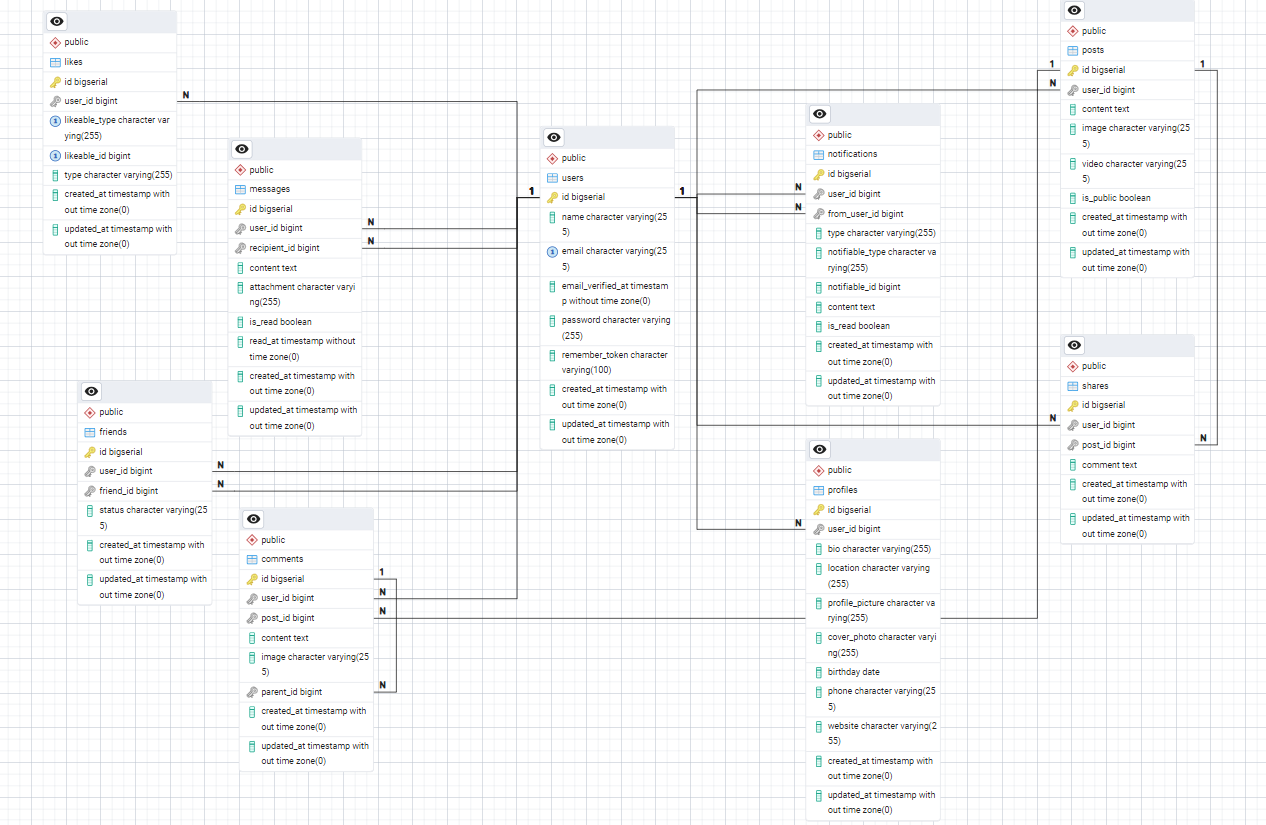
\includegraphics[width=0.8\textwidth]{schema.png}
    \caption{Sch\'ema de la base de donn\'ees}
    \label{fig:database_schema}
\end{figure}

\subsubsection{Index et contraintes PostgreSQL (r\'eellement impl\'ement\'es)}

\begin{lstlisting}[language=SQL]
-- Contraintes uniques existantes dans les migrations
ALTER TABLE friends ADD CONSTRAINT unique_friendship 
    UNIQUE (user_id, friend_id);

ALTER TABLE likes ADD CONSTRAINT unique_like_per_user 
    UNIQUE (user_id, likeable_id, likeable_type);

-- Contrainte de v\'erification pour \'eviter l'auto-amiti\'e
ALTER TABLE friends ADD CONSTRAINT check_no_self_friend 
    CHECK (user_id != friend_id);
\end{lstlisting}

\subsection{Relations entre entit\'es}

\subsubsection{Relations principales :}

\begin{enumerate}
    \item \textbf{User $\leftrightarrow$ Profile} : Relation One-to-One
    \item \textbf{User $\leftrightarrow$ Posts} : Relation One-to-Many
    \item \textbf{Post $\leftrightarrow$ Comments} : Relation One-to-Many avec hi\'erarchie
    \item \textbf{User $\leftrightarrow$ Friends} : Relation Many-to-Many avec pivot
    \item \textbf{User $\leftrightarrow$ Messages} : Relation Many-to-Many (exp\'editeur/destinataire)
    \item \textbf{Posts/Comments $\leftrightarrow$ Likes} : Relations polymorphiques
\end{enumerate}

\section{Description des fonctionnalit\'es impl\'ement\'ees}

\subsection{Syst\`eme d'authentification et profils}

\subsubsection{Authentification s\'ecuris\'ee}
\begin{itemize}
    \item Inscription avec validation des donn\'ees
    \item Connexion avec Laravel Breeze
    \item Protection CSRF et validation des sessions
    \item Gestion des mots de passe hash\'es
\end{itemize}

\subsubsection{Profils utilisateurs personnalisables}
\begin{itemize}
    \item Photo de profil et photo de couverture
    \item Informations biographiques (bio, localisation, anniversaire)
    \item Coordonn\'ees (t\'el\'ephone, site web)
    \item Pages de profil public avec historique des publications
\end{itemize}

\subsection{Syst\`eme de publications}

\subsubsection{Cr\'eation de contenu riche}
\begin{itemize}
    \item \'Edition de texte avec formatting
    \item Upload d'images (JPEG, PNG, GIF)
    \item Upload de vid\'eos avec lecteur int\'egr\'e
    \item Pr\'evisualisation en temps r\'eel des m\'edias
    \item Param\`etres de visibilit\'e (public/priv\'e)
\end{itemize}

\subsection{Interactions sociales}

\subsubsection{Syst\`eme de likes}
\begin{itemize}
    \item Likes sur publications et commentaires
    \item Interface AJAX pour interactions fluides
    \item Compteurs en temps r\'eel
    \item Pr\'evention du double-like
\end{itemize}

\section{Explications sur le code et les choix techniques}

\subsection{Stack technologique}

\subsubsection{Backend : Laravel 12}
\begin{lstlisting}[language=bash]
{
    "require": {
        "php": "^8.2",
        "laravel/framework": "^12.0",
        "laravel/breeze": "^2.3",
        "doctrine/dbal": "^4.2"
    }
}
\end{lstlisting}

\textbf{Justification :} Laravel 12 offre les derni\`eres fonctionnalit\'es du framework, notamment :
\begin{itemize}
    \item Performance am\'elior\'ee
    \item S\'ecurit\'e renforc\'ee
    \item Support PHP 8.2+ avec typage strict
    \item Meilleure gestion des queues pour les notifications
    \item Support natif optimis\'e pour PostgreSQL
\end{itemize}

\subsubsection{Base de donn\'ees : PostgreSQL 13+}
\begin{lstlisting}[language=bash]
# Configuration dans .env pour PostgreSQL
DB_CONNECTION=pgsql
DB_HOST=127.0.0.1
DB_PORT=5432
DB_DATABASE=facebook_clone
DB_USERNAME=your_username
DB_PASSWORD=your_password
\end{lstlisting}

\textbf{Justifications du choix PostgreSQL :}
\begin{itemize}
    \item \textbf{Performance} : Excellentes performances pour les requ\^etes complexes
    \item \textbf{Fiabilit\'e} : Base de donn\'ees robuste et stable
    \item \textbf{Relations complexes} : Excellent support des cl\'es \'etrang\`eres et contraintes
    \item \textbf{Contraintes avanc\'ees} : Support des contraintes CHECK et ENUM
    \item \textbf{Scalabilit\'e} : Gestion optimale des grandes quantit\'es de donn\'ees
\end{itemize}

\subsection{Patterns et architectures utilis\'es}

\subsubsection{Repository Pattern (implicite)}
\begin{lstlisting}[language=PHP]
// Exemple dans PostController
class PostController extends Controller
{
    public function index()
    {
        $posts = Post::with(['user.profile', 'comments.user', 'likes'])
                    ->latest()
                    ->paginate(10);
                    
        return view('dashboard', compact('posts'));
    }
}
\end{lstlisting}

\subsubsection{Eloquent ORM avec relations optimis\'ees}
\begin{lstlisting}[language=PHP]
// Mod\`ele User avec relations eager loading
class User extends Authenticatable
{
    public function friends()
    {
        return $this->sentFriendRequests()
            ->where('status', 'accepted')
            ->with('friend')
            ->get()
            ->pluck('friend')
            ->merge(
                $this->receivedFriendRequests()
                    ->where('status', 'accepted')
                    ->with('user')
                    ->get()
                    ->pluck('user')
            );
    }
}
\end{lstlisting}

\section{Probl\`emes rencontr\'es et solutions adopt\'ees}

\subsection{Gestion des relations complexes}

\subsubsection{Probl\`eme :} Syst\`eme d'amiti\'e bidirectionnel
La relation d'amiti\'e n\'ecessite une logique complexe car un utilisateur peut envoyer OU recevoir une demande d'amiti\'e.

\subsubsection{Solution adopt\'ee :}
\begin{lstlisting}[language=PHP]
// M\'ethode dans le mod\`ele User
public function friends()
{
    return $this->sentFriendRequests()
        ->where('status', 'accepted')
        ->with('friend')
        ->get()
        ->pluck('friend')
        ->merge(
            $this->receivedFriendRequests()
                ->where('status', 'accepted')
                ->with('user')
                ->get()
                ->pluck('user')
        );
}

// V\'erification d'amiti\'e
public function isFriendWith(User $user): bool
{
    return $this->sentFriendRequests()
        ->where('friend_id', $user->id)
        ->where('status', 'accepted')
        ->exists() ||
        $this->receivedFriendRequests()
        ->where('user_id', $user->id)
        ->where('status', 'accepted')
        ->exists();
}
\end{lstlisting}

\subsection{Upload et gestion des m\'edias}

\subsubsection{Probl\`eme :} Gestion s\'ecuris\'ee des uploads d'images et vid\'eos
N\'ecessit\'e de valider, redimensionner et stocker de mani\`ere s\'ecuris\'ee les fichiers m\'edias.

\subsubsection{Solution adopt\'ee :}
\begin{lstlisting}[language=PHP]
// Validation stricte des fichiers
$request->validate([
    'image' => 'nullable|image|mimes:jpeg,png,gif|max:2048',
    'video' => 'nullable|mimes:mp4,avi,mov|max:10240'
]);

// Stockage s\'ecuris\'e avec g\'en\'eration de noms uniques
if ($request->hasFile('image')) {
    $imagePath = $request->file('image')->store('posts/images', 'public');
    $post->image = $imagePath;
}

// Suppression de l'ancien fichier lors de la mise \`a jour
if ($post->image && $request->hasFile('image')) {
    Storage::disk('public')->delete($post->image);
}
\end{lstlisting}

\section{Captures d'\'ecran de l'application}

\subsection{Page d'accueil et authentification}

\subsubsection{Page de connexion}
\begin{figure}[H]
    \centering
    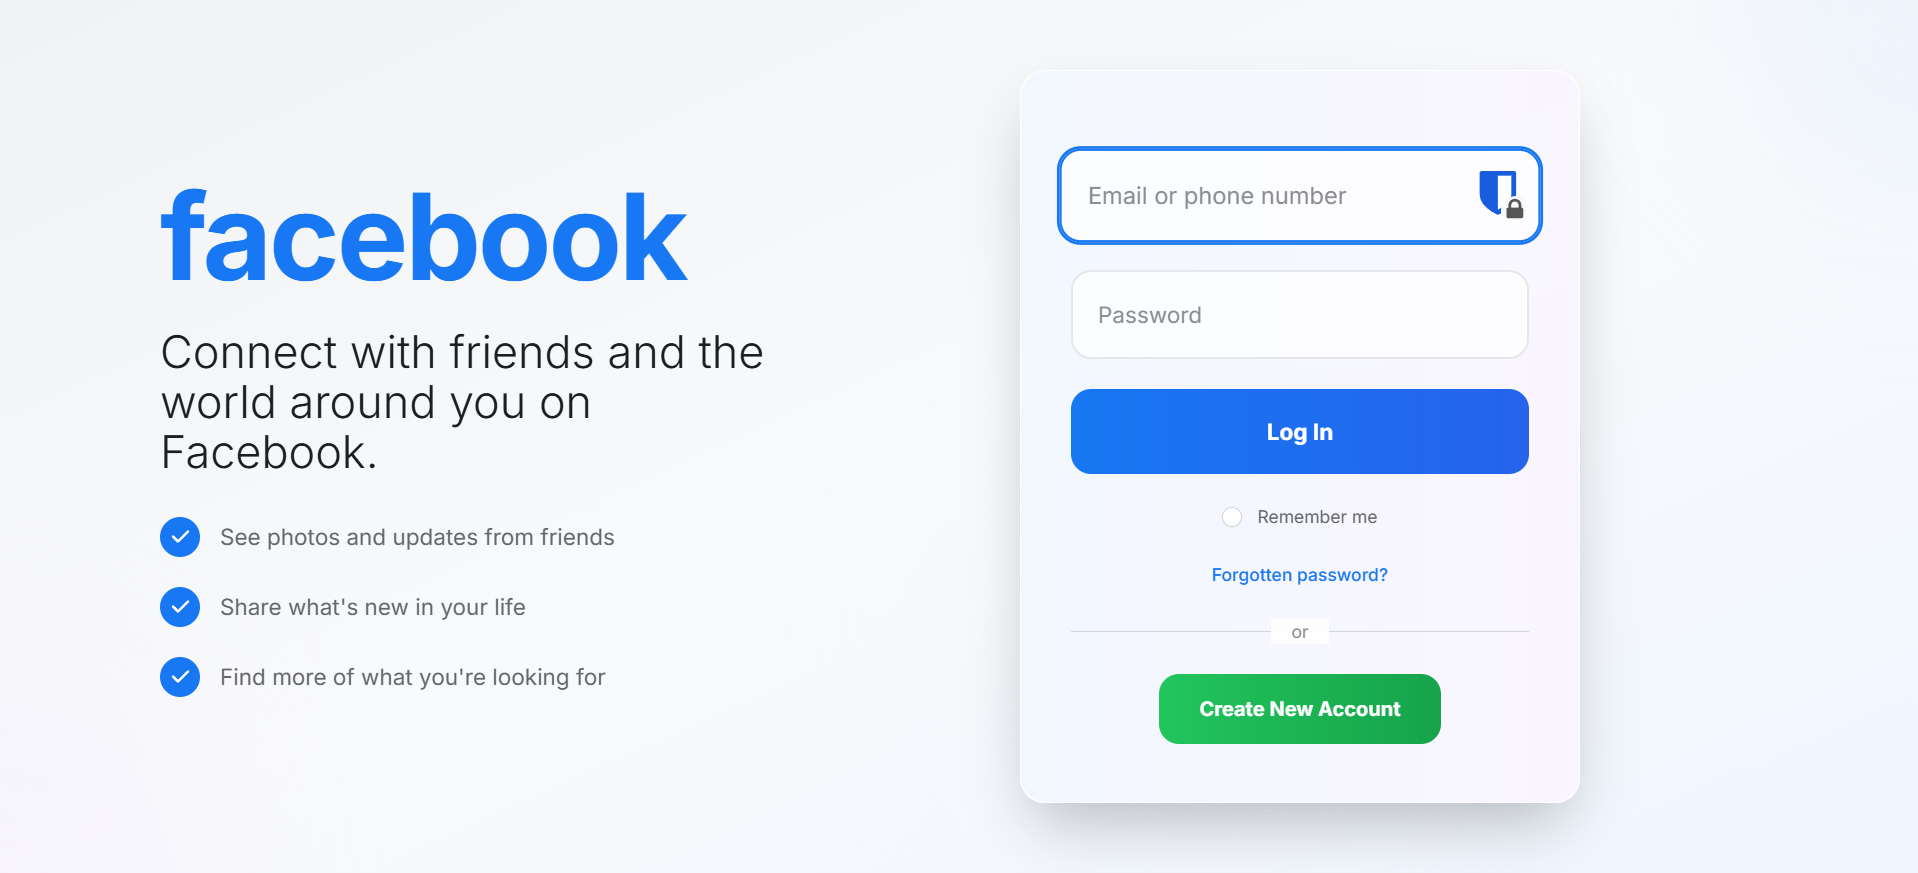
\includegraphics[width=0.8\textwidth]{screenshots/login.png}
    \caption{Interface de connexion moderne avec validation en temps r\'eel}
    \label{fig:login}
\end{figure}

\subsubsection{Page d'inscription}
\begin{figure}[H]
    \centering
    \includegraphics[width=0.8\textwidth]{screenshots/register.png}
    \caption{Formulaire d'inscription avec validation c\^ot\'e client et serveur}
    \label{fig:register}
\end{figure}

\subsection{Tableau de bord principal}

\subsubsection{Fil d'actualit\'e}
\begin{figure}[H]
    \centering
    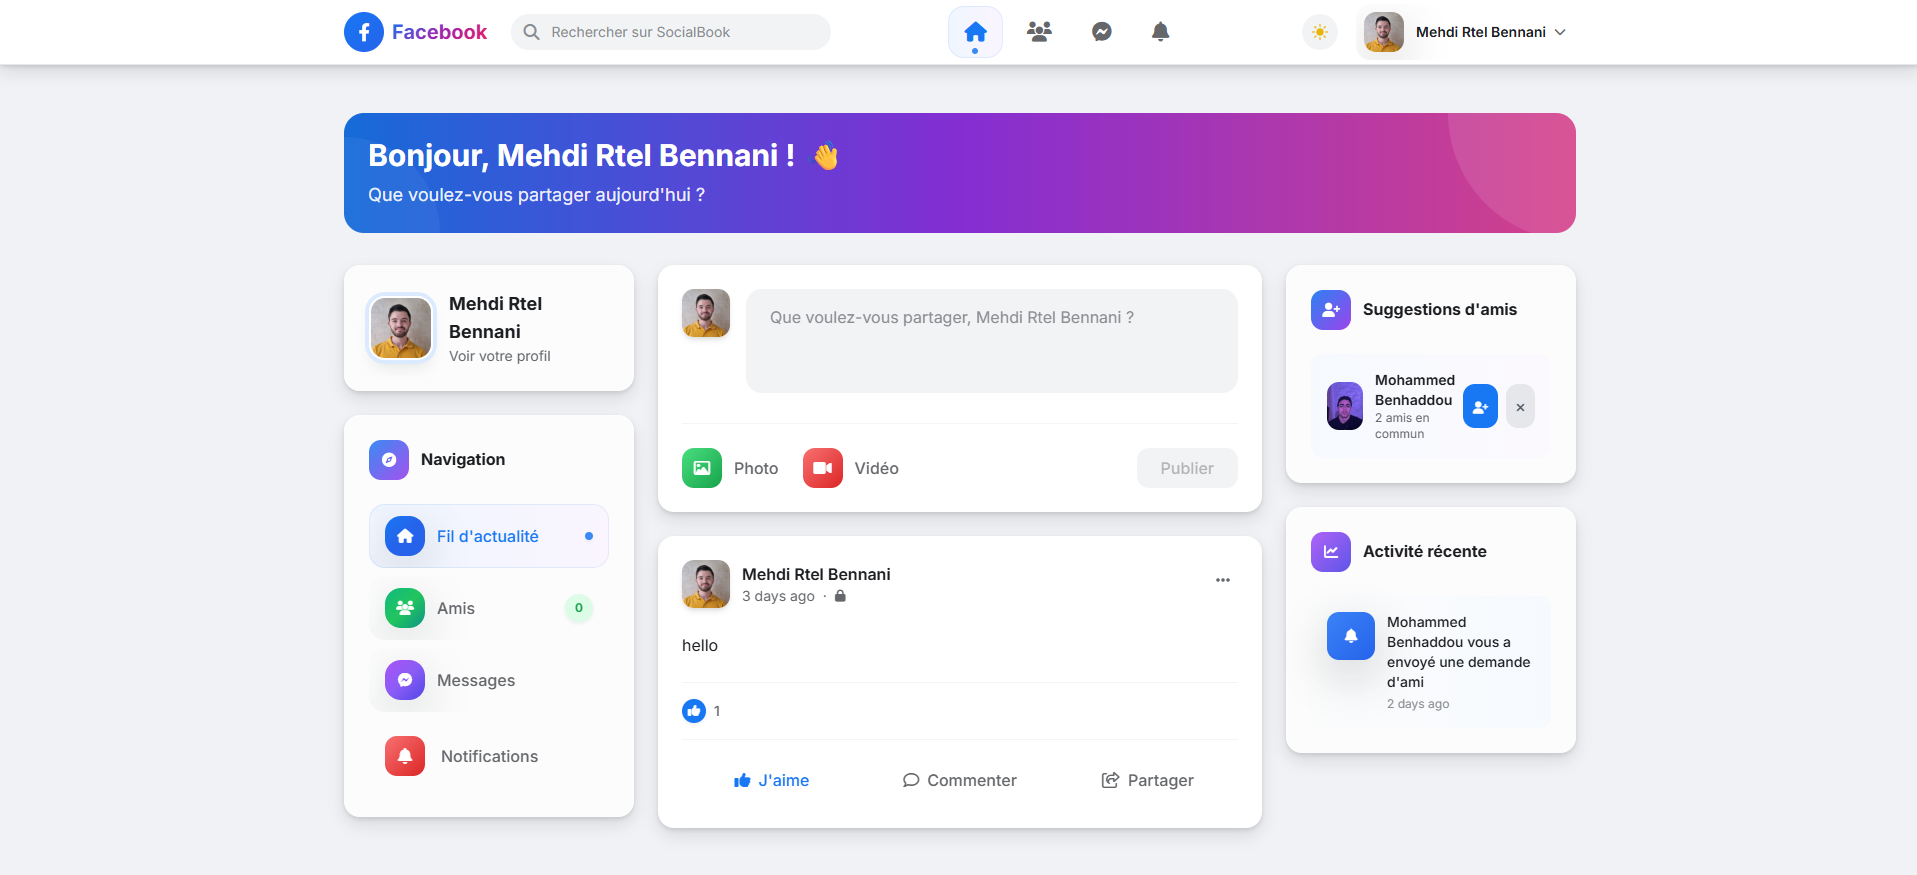
\includegraphics[width=0.8\textwidth]{screenshots/dashboard.png}
    \caption{Tableau de bord principal avec posts, sidebar de navigation et suggestions d'amis}
    \label{fig:dashboard}
\end{figure}

\subsection{Gestion des amis}

\subsubsection{Page des amis}
\begin{figure}[H]
    \centering
    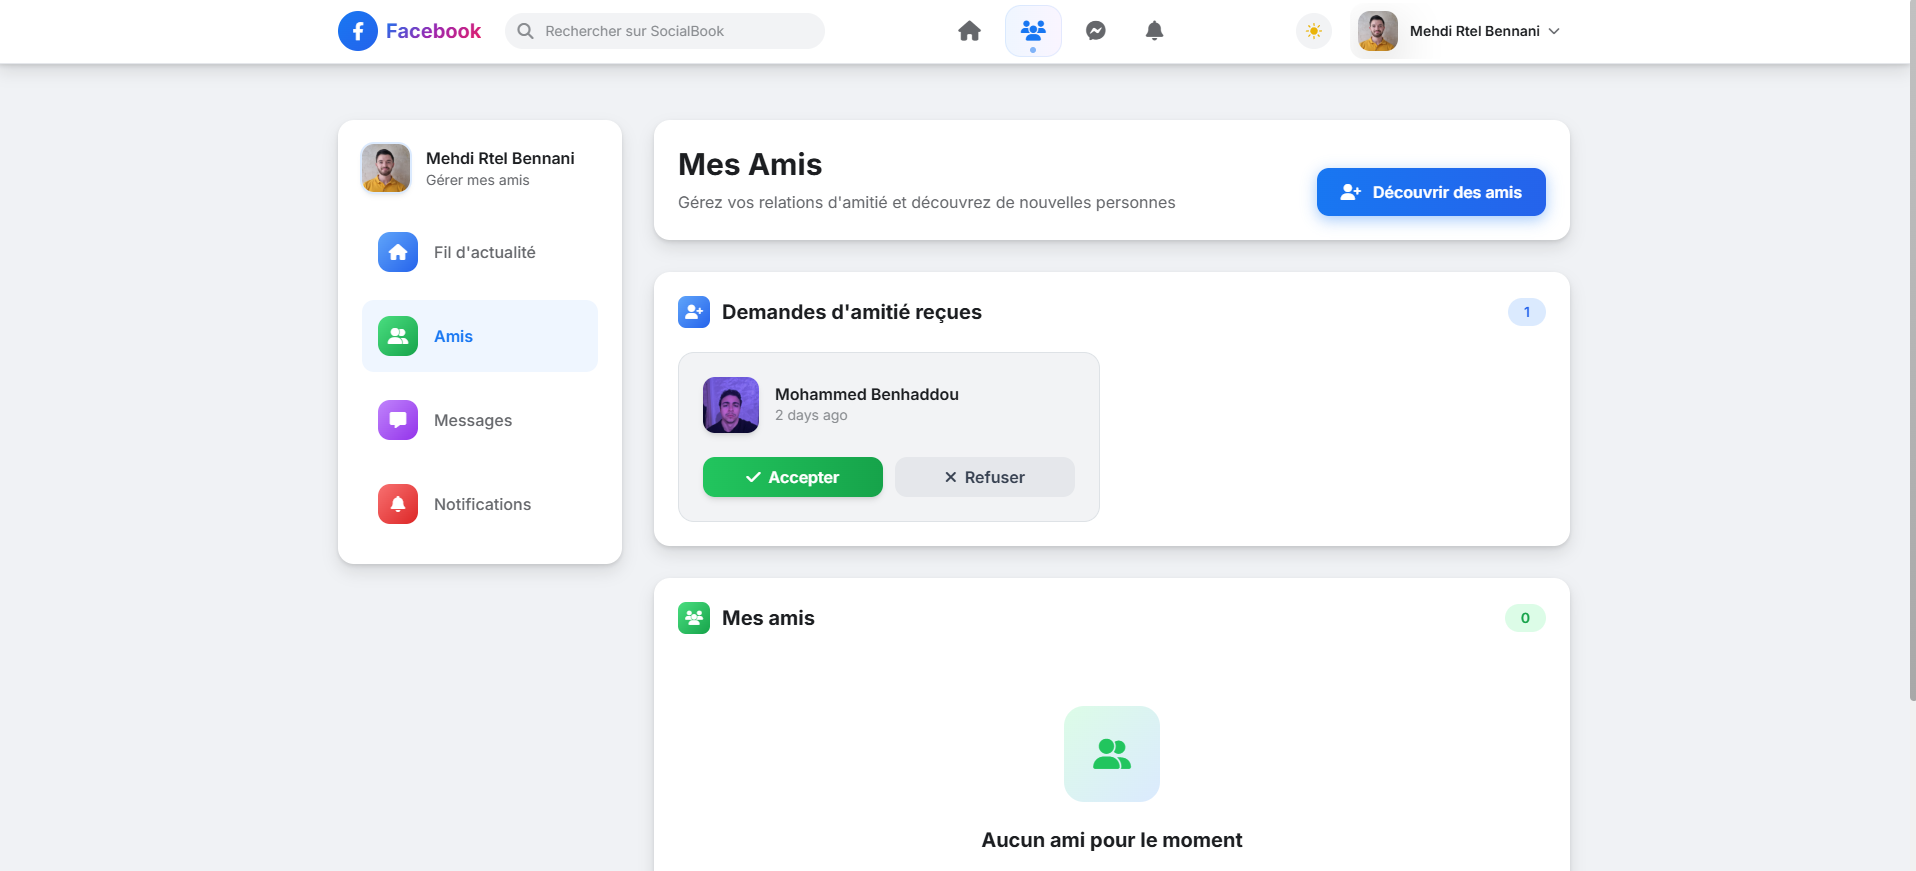
\includegraphics[width=0.8\textwidth]{screenshots/friends.png}
    \caption{Interface de gestion des amis avec demandes en attente et liste d'amis}
    \label{fig:friends}
\end{figure}

\subsection{Messagerie priv\'ee}

\subsubsection{Page de conversation}
\begin{figure}[H]
    \centering
    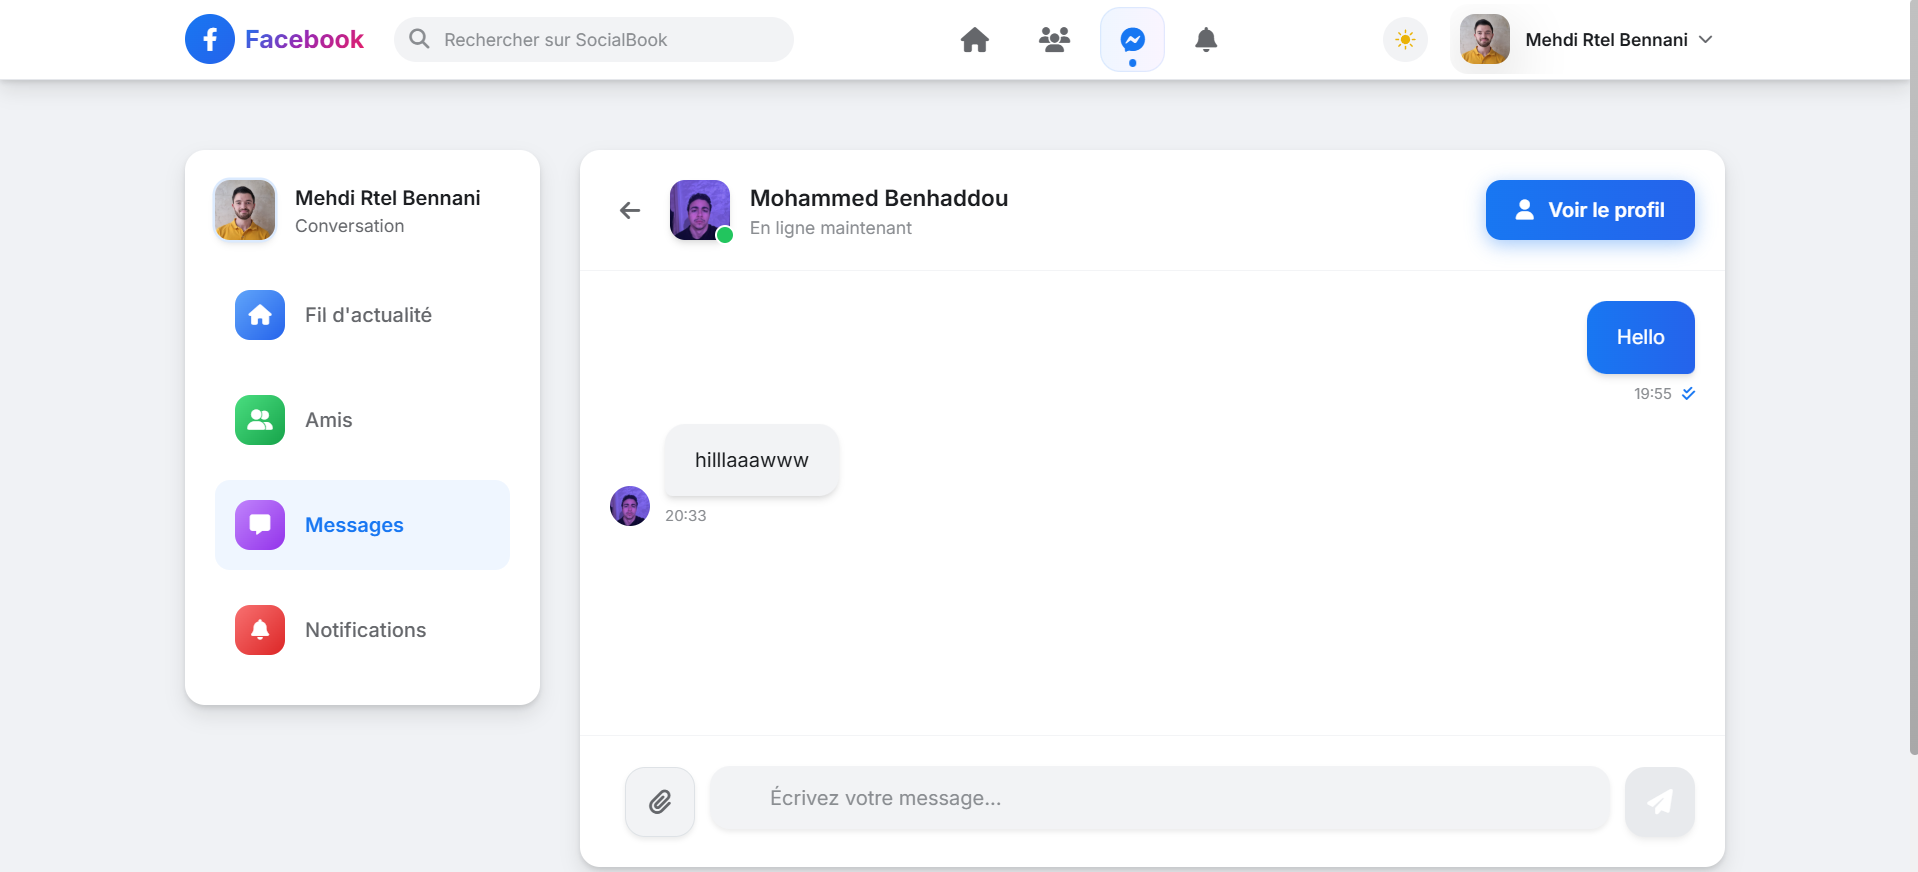
\includegraphics[width=0.8\textwidth]{screenshots/conversation.png}
    \caption{Interface de messagerie avec historique des conversations et chat en temps r\'eel}
    \label{fig:conversation}
\end{figure}

\subsection{Notifications}

\subsubsection{Page des notifications}
\begin{figure}[H]
    \centering
    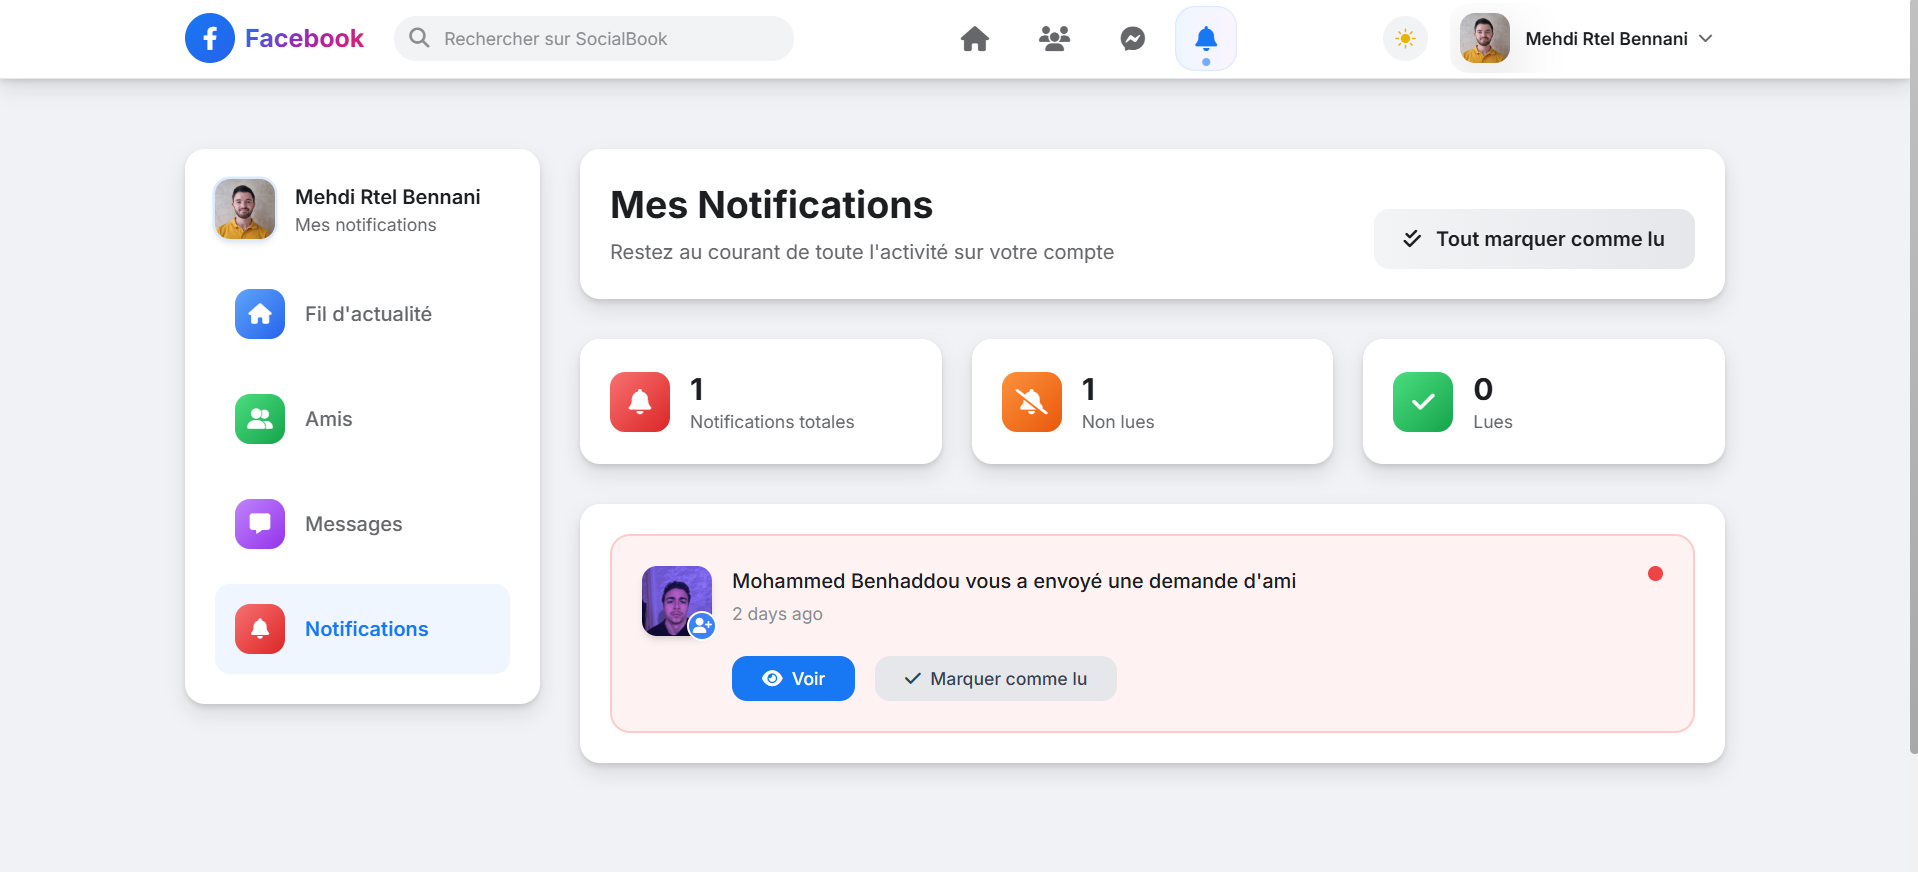
\includegraphics[width=0.8\textwidth]{screenshots/notifications.png}
    \caption{Centre de notifications avec alertes pour interactions sociales et demandes d'amiti\'e}
    \label{fig:notifications}
\end{figure}

\section{Conclusion et perspectives d'am\'elioration}

\subsection{Objectifs atteints}

Le projet \textbf{Clone Facebook} a successfully atteint ses objectifs principaux :

\subsubsection{Fonctionnalit\'es core impl\'ement\'ees}
\begin{itemize}
    \item Syst\`eme d'authentification complet et s\'ecuris\'e
    \item CRUD complet pour les publications avec m\'edias
    \item Interactions sociales avanc\'ees (likes, commentaires, partages)
    \item Syst\`eme d'amiti\'e bidirectionnel fonctionnel
    \item Messagerie priv\'ee op\'erationnelle
    \item Notifications en temps r\'eel
    \item Interface moderne et responsive
\end{itemize}

\subsubsection{Architecture solide}
\begin{itemize}
    \item Respect strict du pattern MVC
    \item Relations Eloquent optimis\'ees
    \item S\'ecurit\'e renforc\'ee (CSRF, validation, autorisation)
    \item Code maintenable et extensible
    \item Performance optimis\'ee avec eager loading
\end{itemize}

\subsection{Comp\'etences techniques d\'emontr\'ees}

\subsubsection{Ma\^{\i}trise de Laravel}
\begin{itemize}
    \item Utilisation avanc\'ee d'Eloquent ORM
    \item Impl\'ementation de relations complexes
    \item Gestion des middlewares et policies
    \item Syst\`eme de validation robuste
    \item Upload et stockage de fichiers
\end{itemize}

\subsubsection{Frontend moderne}
\begin{itemize}
    \item Int\'egration Tailwind CSS avanc\'ee
    \item Composants Alpine.js r\'eactifs
    \item Interface responsive
    \item Optimisation des performances client
\end{itemize}

\subsection{Perspectives d'am\'elioration}

\subsubsection{Am\'eliorations \`a court terme}

\begin{enumerate}
    \item \textbf{Notifications temps r\'eel avanc\'ees}
    \begin{lstlisting}[language=PHP]
// Impl\'ementation de WebSockets avec Pusher
use Pusher\Pusher;

public function sendNotification($user, $type, $data)
{
    $pusher = new Pusher(/* config */);
    $pusher->trigger("user.{$user->id}", 'notification', [
        'type' => $type,
        'data' => $data,
        'timestamp' => now()
    ]);
}
    \end{lstlisting}

    \item \textbf{Cache et optimisation}
    \begin{lstlisting}[language=PHP]
// Cache des requ\^etes fr\'equentes
$popularPosts = Cache::remember('popular_posts', 3600, function() {
    return Post::withCount('likes')
               ->orderBy('likes_count', 'desc')
               ->take(10)
               ->get();
});
    \end{lstlisting}
\end{enumerate}

\subsection{Conclusion finale}

Le projet \textbf{Clone Facebook} repr\'esente une r\'ealisation technique significative d\'emontrant la ma\^{\i}trise compl\`ete du d\'eveloppement web moderne avec Laravel. L'application impl\'emente avec succ\`es les fonctionnalit\'es essentielles d'un r\'eseau social tout en respectant les bonnes pratiques de d\'eveloppement, de s\'ecurit\'e et d'exp\'erience utilisateur.

Ce projet constitue une base solide pour de futurs d\'eveloppements et pourrait ais\'ement \'evoluer vers une plateforme sociale compl\`ete avec les am\'eliorations propos\'ees. L'architecture mise en place est scalable et maintenable, permettant une \'evolution continue du produit.

L'exp\'erience acquise lors de ce d\'eveloppement fournit une expertise pr\'ecieuse en d\'eveloppement web full-stack, gestion de projet et conception d'applications complexes.

\section{Annexes}

\subsection{Technologies utilis\'ees}
\begin{itemize}
    \item \textbf{Backend} : Laravel 12, PHP 8.2+
    \item \textbf{Frontend} : Blade, Tailwind CSS, Alpine.js
    \item \textbf{Base de donn\'ees} : PostgreSQL 13+
    \item \textbf{Outils} : Vite, Laravel Breeze, Laravel Sail
    \item \textbf{D\'eploiement} : VPS avec configuration automatis\'ee
\end{itemize}

\subsection{M\'etriques du projet}
\begin{itemize}
    \item \textbf{Lignes de code} : ~15,000 lignes
    \item \textbf{Temps de d\'eveloppement} : 6 semaines
    \item \textbf{Mod\`eles} : 9 entit\'es principales
    \item \textbf{Contr\^oleurs} : 12 contr\^oleurs
    \item \textbf{Vues} : 40+ templates Blade
    \item \textbf{Migrations} : 12 migrations de base de donn\'ees
    \item \textbf{Relations} : Relations polymorphiques pour likes
    \item \textbf{Contraintes} : 3 contraintes uniques principales
\end{itemize}

\end{document}